%%%%%%%%%%%%%%%%%%%%%%%%%%%%%%%%%%%%%%%%%%%%%%%%%%%%%%%%%%%%%%%%%%%%%%%%%%%%%%%%
%2345678901234567890123456789012345678901234567890123456789012345678901234567890
%        1         2         3         4         5         6         7         8

\documentclass[letterpaper, 10 pt, conference]{ieeeconf}  % Comment this line out if you need a4paper

%\documentclass[a4paper, 10pt, conference]{ieeeconf} % Use this line for a4 paper

% \IEEEoverridecommandlockouts %This command is only needed if you want to use the \thanks command

\overrideIEEEmargins  % Needed to meet printer requirements.

%In case you encounter the following error:
%Error 1010 The PDF file may be corrupt (unable to open PDF file) OR
%Error 1000 An error occurred while parsing a contents stream. Unable to analyze the PDF file.
%This is a known problem with pdfLaTeX conversion filter. The file cannot be opened with acrobat reader
%Please use one of the alternatives below to circumvent this error by uncommenting one or the other
%\pdfobjcompresslevel=0
%\pdfminorversion=4

% See the \addtolength command later in the file to balance the column lengths
% on the last page of the document

% The following packages can be found on http:\\www.ctan.org
\usepackage{graphicx} % for pdf, bitmapped graphics files
%\usepackage{epsfig} % for postscript graphics files
%\usepackage{mathptmx} % assumes new font selection scheme installed
%\usepackage{times} % assumes new font selection scheme installed
\usepackage{amsmath} % assumes amsmath package installed
\usepackage{amssymb}  % assumes amsmath package installed
%\usepackage{dsfont}
\usepackage{algorithm}
\usepackage{algorithmic}
\usepackage{commath}

\usepackage{xcolor}
\newcommand{\todo}[1]{{\color{blue}[TODO: #1]}}
\newcommand{\response}[1]{{\color{green}[RESPONSE: #1]}}
\graphicspath{{figures/}}


\DeclareMathOperator*{\argmax}{arg\,max}
\DeclareMathOperator*{\argmin}{arg\,min}

\title{\LARGE \bf
Multi-Agent Autonomous Mapping of Unknown GPS-Denied Environments Using a Relative Navigation Framework}

\author{Jacob M. Olson$^{1}$, Timothy W. McLain$^{2}$ \todo{include Matthiew Labbe?}% <-this % stops a space
%\thanks{This research was supported through the Center for Unmanned Aircraft Systems (C-UAS), a National Science Foundation-sponsored industry/university cooperative research center (I/UCRC) under NSF Award No. IIP-1650547 along with significant contributions from C-UAS industry members.}% <-this % stops a space
\thanks{$^{1}$The corresponding author can be contacted at
        {\tt\small jacobmo at byu.edu}.}%
\thanks{$^{2}$All authors are with the Department of Mechanical Engineering or Electrical and Computer Engineering,
        Brigham Young University, Provo, UT, 84602, USA.}%
%\thanks{$^{3}$C. Peterson is with the Faculty of Electrical and Computer Engineering,
%		Brigham Young University, Provo, UT, 84602, USA.
%        {\tt\small cammy.peterson at byu.edu}}%
%\thanks{$^{4}$R. W. Beard is with the Faculty of Electrical and Computer Engineering,
%		Brigham Young University, Provo, UT, 84602, USA.
%        {\tt\small beard at byu.edu}}%
}

\begin{document}

\maketitle
\thispagestyle{empty}
\pagestyle{empty}


%%%%%%%%%%%%%%%%%%%%%%%%%%%%%%%%%%%%%%%%%%%%%%%%%%%%%%%%%%%%%%%%%%%%%%%%%%%%%%%%
\begin{abstract}

\todo{write the abstract}

\end{abstract}


%%%%%%%%%%%%%%%%%%%%%%%%%%%%%%%%%%%%%%%%%%%%%%%%%%%%%%%%%%%%%%%%%%%%%%%%%%%%%%%%
\section{Introduction}

The remainder of the paper is organized as follows: Section \ref{approach} describes framework used to map the environment and background on what previous work has made this research possible. Section \ref{planning} details the planning and control schemes used to successfully navigate the unknown area. Then method used to combine maps of multiple agents are then explained in Section \ref{merge}. Results showing and evaluating the generated maps are presented in Section \ref{results}. Finally, conclusions are presented in Section \ref{conclusions}.

%%%%%%%%%%%%%%%%%%%%%%%%%%%%%%%%%%%%%%%%%%%%%%%%%%%%%%%%%%%%%%%%%%%%%%%%%%%%%%%%
\section{Technical Approach}\label{approach}

\subsection{Problem Statement}

The goal of this project is to successfully map a GPS-denied environment using multiple UAVs collaborating with eachother to explore the environment. This framework assumes that a good set of high level waypoints will be provided that ensure sufficient loop closures and coverage of the desired area. The focus in this paper is properly estimating the UAV states to allow for successful GPS-denied navigation and map merging. The network diagram showing the framework used is shown in Fig. \ref{fig:rtab_network} which will be described in detail in this section and throughout the paper.

\begin{figure*}
\centering
\includegraphics[width=1.0\linewidth]{rtab_relative_nav_network}
\caption{The network diagram of the relative navigation framework proposed in this paper}
\label{fig:rtab_network}
\end{figure*}

\subsection{Sensors}

Since we are operating in a GPS-denied environment, we are not able to rely on GPS measurements to give us global information about where the UAVs are located. As shown in Fig. \ref{fig:rtab_network} the sensors used by the UAV to estimate its state are an RGB-D camera, a planar laser scanner, a LiDAR pencil-beam sensor and an IMU on the onboard flight controller. Using only these sensors and the flight computer, we must be able to accurately estimate the states of the UAV enough to send waypoints and control the attitude. Since global position is not measurable and must be estimated, it is important to not rely on the current global estimates for attitude control. \todo{how much do I talk about sensors here?}

\subsection{Estimation}

Estimation is the most critical element in enabling autonomous flight. Without good position and attitude estimation, autonomous navigation algorithms do not function. To avoid the issue of loop closures causing instability in the controller, we separately estimate the global and relative position and do not directly rely on the global estimate to control the attitude of the UAV. The current estimates are stored in a transformation tree as shown in Fig. \ref{fig:tf_tree}. The world frame is the inertial NED frame of the world with a static transform to the map frame. The map frame is a NWU frame set by RTAB-Map as in the starting location where it is initialized. RTAB-Map uses the odom fram to adjust for loop closures without causing spikes in the odometry. The odom frame starts with zero transformation from the map frame. Each time a new loop closure is detected, if the map optimization shifts the global position estimate, rather than alter the odometry message, causing spikes in the estimated odometry, the entire tree from odom down is shifted with the loop closure adjustment. Every time RTAB-Map creates a new node in the graph, the visual odometry node resets the keyframe transform to the current base-link transform. the base-link transform represents the current estimated position of the the UAV in the NED frame and camera-link represents the position in the NWU frame, the camera-base-link transform represents the current position of the camera in the camera frame. the waypoint manager drops the current waypoint connected to the world frame. This way a loop closure does not shift the desired gloabal position of the waypoint. The position controller controls on the error between the waypoint and base-link. This is under the assumption that the desired waypoint location is known globaly, this could be modified to set the new waypoint relative to odom frame if the position is relative to the current obstacles rather than the global position.

\begin{figure*}
\centering
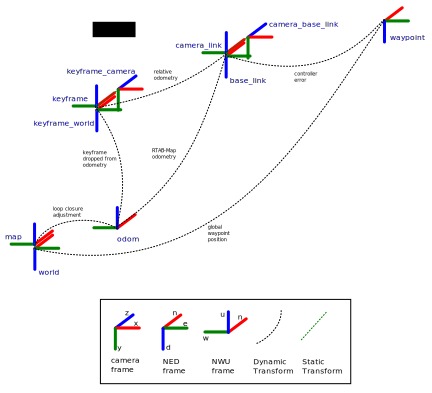
\includegraphics[width=0.9\linewidth]{tf_tree_relative_rtab}
\caption{The transformation tree of the reference frames used in estimation and control.}
\label{fig:tf_tree}
\end{figure*}

\subsubsection{RTAB-Map}

RTAB-Map is a powerful open source software package that uses graph-based SLAM with appearence based loop closures to generate high-quality, dense 3D maps of environments without the use of GPS. RTAB-Map is also able to accurately estimate position within the map with little error. \todo{cite RTAB-Map papers} We use the visual odometry from RTAB-Map as an input to the estimation for the relative framework. We directly use the current global estimate of RTAB-Map for the position controller and waypoint manager.

RTAB-Map has been extended to build a single map from multiple different sessions at different times, but currently is not able to handle simultaneous multi-agent mapping. This paper proposes a method to extend the functionality of RTAB-Map to combine the maps of multiple agents flying simultaneously into a single map in near real time.

RTAB map does not estimate the attitude of a UAV with enough frequency to autonomously navigate so we used the relative navigation framework to estimate attitude and relative state.

\subsubsection{Visual Odometry}

The odometry and keyframe information from RTAB-Map is used to generate a relative odometry message that is used by the relative estimator. RTAB-Map produces a global visual odometry. the visual odometry node publishes only the translation and rotation from the last keyframe that has been dropped. when RTAB-Map begins a new keyframe, the relative odometry message flags the keyframe change and resets the relative odometry. this makes it so that the large global position jumps caused by loop closure do not translate into the relative odometry and it is only tracking the transform between keyframes.

\subsubsection{RMEKF}
The Relative Multiplicative Extended Kalman Filter (RMEKF) was shown to successfully estimate the UAV's relative state sufficient to autonomously navigate in GPS-denied environments that had been previously mapped. Thus far, however, it has not been extended to estimation and navigation in unknown and unmapped environments, this paper proposes a method to extend the functionality to these environments.

The RMEKF takes as inputs the IMU measurement from the flight controller, the relative visual odometry based on a keyframe approach, and the attitude measurement from the LiDAR pencil beam sensor. Then using the multirotor dynamics model, is able to accurately estimate the relative state of the UAV. It is important to note that the RMEKF makes no effort to estimate the global position of the UAV. This makes it so that large corrections in the estimated global position that happen with loop closures do not cause the estimator to diverge, and therefore cause stability issues in the velocity and attitude controllers onboard the UAV. The RMEKF functionality and results are further detailed in \todo{cite relative nav papers}.

\subsection{Control}

To sucessfully control a UAV in a GPS-denied environment, the control must be segmented into different categories to take advantage of both global and relative estimates. The control scheme cascades from an input map, current estimated position, and current goal position and outputs the motor commands at the end.

\subsubsection{Waypoint Planner}

The first stage of the control is the waypoint planner. It takes the global goal, current known obstacles, and current global estimates as obstacles and outputs a set of waypoints to reach the goal while avoiding the current waypoints. This stage will be further explained in Section \ref{planning}.

\subsubsection{Waypoint Manager}

After receiving the current set of waypoints, the waypoint manager selects the appropriate waypoint for the UAV to fly towards and sends the global location to the position controller. The waypoint manager monitors the position and angle error between the current estimated position and the current waypoint and when the error crosses below a user-defined threshold value, the next waypoint is sent to the position controller.

\subsubsection{Position Controller}

The position controller controls on the error between the current estimated position of the UAV and the next waypoint. The goal of the position controller is to drive the error to zero. Since it operates in the error space of the the UAV rather than the state space, sudden shifts in the UAVs position estimate caused by loop closures have minimal effect on the controller and it is able to continue controlling the error to zero. The output of the position controller is a velocity command for the UAV.

\subsubsection{Obstacle Avoidance}

Before passing the velocity control into the attitude controller, it is filtered through an obstacle avoidance node as described in \todo{cite obstacle avoidance}, which uses the current relative estimates and obstacles detected py the planar laser scanner and using a potential fields method pushes away from obstacles and towards the commanded velocity input. The obstacle avoidance node then sends the modified velocity command to the attitude controller. 

\subsubsection{Rotor Controller}

\subsection{Inputs/Outputs}


%%%%%%%%%%%%%%%%%%%%%%%%%%%%%%%%%%%%%%%%%%%%%%%%%%%%%%%%%%%%%%%%%%%%%%%%%%%%%%%%
\section{Planning}\label{planning}

\subsection{Global Goal Following with Relative Estimation}

\subsection{Reactive Path Planning}

\begin{figure*}
\centering
\includegraphics[width=1.0\linewidth]{adaptive_path_plan2.png}
\caption{An example of how the reactive path planner works as the UAV flies the planned path. The current estimated position is marked by the green arrow, the current goal position is marked by the red arrow, and the current path planned is marked with the blue lines. Detected obstacles with their respective safety buffers are represented with black and grey respectively.}
\label{fig:reactive_plan}
\end{figure*}

%%%%%%%%%%%%%%%%%%%%%%%%%%%%%%%%%%%%%%%%%%%%%%%%%%%%%%%%%%%%%%%%%%%%%%%%%%%%%%%%
\section{Map Merging}\label{merge}

\begin{figure*}
\centering
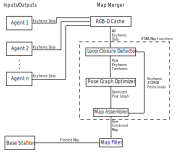
\includegraphics[width=0.7\linewidth]{map_merger_network}
\caption{The network diagram for the multi-agent map merging node proposed in this section.}
\label{fig:map_merge}
\end{figure*}
%%%%%%%%%%%%%%%%%%%%%%%%%%%%%%%%%%%%%%%%%%%%%%%%%%%%%%%%%%%%%%%%%%%%%%%%%%%%%%%%
\section{Results and Discussion}\label{results}

\subsection{Simulation}

\subsection{Hardware}
%%%%%%%%%%%%%%%%%%%%%%%%%%%%%%%%%%%%%%%%%%%%%%%%%%%%%%%%%%%%%%%%%%%%%%%%%%%%%%%%
\section{Conclusions}\label{conclusions}


%%%%%%%%%%%%%%%%%%%%%%%%%%%%%%%%%%%%%%%%%%%%%%%%%%%%%%%%%%%%%%%%%%%%%%%%%%%%%%%%

\bibliographystyle{IEEEtran} % We choose the "plain" reference style
\bibliography{mapping_paper_2019}

\end{document}
